% !TeX spellcheck = pt_BR
%%%%%%%%%%%%%%%%%%%%%%%%%%%%%%%%%%%%%%%%%%%%%%%%%%%%%%%%%%%%%%%%%%%%%%%%%%%%%%%%%%%%%%%%%%%%%%%%
%                                                                                              %
%                             Definicao para a classe Artigo                                   %
%                                                                                              %
%%%%%%%%%%%%%%%%%%%%%%%%%%%%%%%%%%%%%%%%%%%%%%%%%%%%%%%%%%%%%%%%%%%%%%%%%%%%%%%%%%%%%%%%%%%%%%%%

\documentclass[portugues, brazil, a4paper,12pt]{article}
\bibliographystyle{plain}

%%%%%%%%%%%%%%%%%%%%%%%%%%%%%%%%%%%%%%%%%%%%%%%%%%%%%%%%%%%%%%%%%%%%%%%%%%%%%%%%%%%%%%%%%%%%%%%%
%                                                                                              %
%                       Pacotes a utilizar na compilacao do documento                          %
%                                                                                              %
%%%%%%%%%%%%%%%%%%%%%%%%%%%%%%%%%%%%%%%%%%%%%%%%%%%%%%%%%%%%%%%%%%%%%%%%%%%%%%%%%%%%%%%%%%%%%%%%

\usepackage[brazil]{babel}
\usepackage{graphicx}
\usepackage{geometry}
\usepackage[utf8]{inputenc}
\usepackage[T1]{fontenc}
\usepackage{algorithm}
\usepackage{color}
\usepackage{minted}
%\usepackage{algorithmic}
\usepackage[noend]{algpseudocode}
\usepackage{epstopdf}
\usepackage{hyperref}
\usepackage{todonotes}
\usepackage{amsmath}
\usepackage{verbatim}
\usepackage{gensymb}

\hypersetup{
    colorlinks,
    citecolor=black,
    filecolor=black,
    linkcolor=black,
    urlcolor=black
}



\makeatletter
\renewcommand{\paragraph}{\@startsection{paragraph}{4}{0ex}%
   {-3.25ex plus -1ex minus -0.2ex}%
   {1.5ex plus 0.2ex}%
   {\normalfont\normalsize\bfseries}}
\makeatother

\stepcounter{secnumdepth}
\stepcounter{tocdepth}

%%%%%%%%%%%%%%%%%%%%%%%%%%%%%%%%%%%%%%%%%%%%%%%%%%%%%%%%%%%%%%%%%%%%%%%%%%%%%%%%%%%%%%%%%%%%%%%%
%                                                                                              %
%                       Configuracao dos pacotes utilizados no doc.                            %
%                                                                                              %
%%%%%%%%%%%%%%%%%%%%%%%%%%%%%%%%%%%%%%%%%%%%%%%%%%%%%%%%%%%%%%%%%%%%%%%%%%%%%%%%%%%%%%%%%%%%%%%%

\geometry{a4paper,left=3cm,right=3cm,top=2.5cm,bottom=2.93cm}


%%%%%%%%%%%%%%%%%%%%%%%%%%%%%%%%%%%%%%%%%%%%%%%%%%%%%%%%%%%%%%%%%%%%%%%%%%%%%%%%%%%%%%%%%%%%%%%%
%                                                                                              %
%                             Capa do relatorio tecnico                                        %
%                                                                                              %
%%%%%%%%%%%%%%%%%%%%%%%%%%%%%%%%%%%%%%%%%%%%%%%%%%%%%%%%%%%%%%%%%%%%%%%%%%%%%%%%%%%%%%%%%%%%%%%%

\begin{document}

\begin{titlepage}

  \vfill

	\begin{figure}[H]
	\centering
		
\includegraphics[scale=0.15]{img/logo-ufop.jpg}
	\end{figure}

  \vfill

  \begin{center}
    \begin{Large}
      \textbf{UNIVERSIDADE FEDERAL DE OURO PRETO}
    \end{Large}
  \end{center}

  \begin{center}
    \begin{large}
      \textbf{Mestrado em Ciência da Computação} \\[1.4cm]
    \end{large}
  \end{center}

  \vfill

  \begin{center}
    \begin{large}
      \textbf{Especificação Sistêmica de Carro Robô Seguidor de Linha com Sistema Avançado Utilizando Controle Proporcional}
    \end{large}
  \end{center}

  \vfill

  \begin{center}
    \begin{large}
      Autor: \\
		Rodolfo Labiapari Mansur Guimarães - \url{rodolfolabiapari@decom.ufop.br}
    \end{large}
  \end{center}

	\vfill

  \begin{center}
    \begin{large}
      Professor: \\
      Ricardo Augusto Rabelo Oliveira - \url{rrabelo@gmail.com}
    \end{large}
  \end{center}

  \vfill

  \begin{center}
    \begin{large}
      Ouro Preto - MG \\
      \today \\
    \end{large}
  \end{center}

\clearpage
\tableofcontents
\end{titlepage}

%%%%%%%%%%%%%%%%%%%%%%%%%%%%%%%%%%%%%%%%%%%%%%%%%%%%%%%%%%%%%%%%%%%%%%%%%%%%%%%%%%%%%%%%%%%%%%%%
%                                                                                              %
%                               Introducao ao trabalho                                         %
%                                                                                              %
%%%%%%%%%%%%%%%%%%%%%%%%%%%%%%%%%%%%%%%%%%%%%%%%%%%%%%%%%%%%%%%%%%%%%%%%%%%%%%%%%%%%%%%%%%%%%%%%
% \textit{hardware} design software designer
\part{Capítulo 3 - \textit{Design} de Sistema}

Segundo Sass, há trinta anos, quando se pensava em sistemas embarcados, falava-se em máquinas computacionais personalizadas construídas a partir de circuitos eletrônicos discretos e integrados. Isso significa que o foco era totalmente em \textit{hardware} e em \textit{design} de \textit{hardware}. O \textit{software}, por sua vez, era somente uma parte do sistema que integrava tudo. Somente produtos fabricados em grande escala justificavam o custo de construir \textit{hardware}s personalizados. Com o passar do tempo a tecnologia foi reduzindo o volume dos componentes sem ter o \textit{trade-off} \footnote{Conflito de escolha. A resolução de problema acarreta noutro.} em vazão e custo e assim era melhor iniciar um projeto com componentes baratos, provendo uma plataforma computacional semi-personalizada. Entretanto, a solução final exigia mais esforço em \textit{software} para gerar uma aplicação para um comportamento específico, e com isso, o desenvolvimento de \textit{software} passou a ser mais custoso que o desenvolvimento em \textit{hardware} tornando-se principal fator no custo de desenvolvimento de um produto.

Dispositivos como Plataformas FPGA quebraram tal situação. Isso pelo fato de que Plataformas FPGAs permitem ao \textit{\textit{design}er} de sistemas embutidos ter uma “lousa branca” e que possa implementar \textit{hardware}s computacionais personalizados tão facilmente como o desenvolvimento de um \textit{software}. Infelizmente, enquanto configurar um FPGA é uma tarefa fácil, criar um \textit{design} de \textit{hardware} inicial não é. Seria inviável implementar toda vez cada \textit{hardware} que fosse necessário em projetos. Por isso, utilizam-se \textit{hardware}s de cores\footnote{} já existentes e desenvolvimento de novos cores para seu re-uso. Basta saber como quais cores serão e como são utilizados, suas performances e como desenvolve novos cores com intuito de deixá-los reutilizáveis.

A partir de então, \textit{\textit{\textit{design}er}s} de Plataformas FPGA devem começar a entender mais sobre desenvolvimento de \textit{software} como sistemas operacionais e dispositivos controladores do que simples aplicações, para trazer o código escrito para a aplicação de fato. Utilizando \textit{hardware}s comerciais, muito desses problemas de plataformas poderiam ser escondidos em sistemas embarcados porque grande parte dos componentes possuem ferramentas e sistemas de baixo nível de \textit{software} para manuseio e dessa forma, ambos \textit{hardware} e \textit{software} agora são programáveis.





\section{Princípios de Design de um Sistema}

Para dar um significado a alguns componentes de \textit{design}, alguns conceitos devem ser definidos a priori.

Para declarar um \textit{design} bom ou ruim, precisa-se definir dois critérios, o critério externo e interno.

Os critérios externos são características que um usuário observaria. Um exemplo é o mau funcionamento de um componente onde em vez de aumentar o volume, é reduzido ao tentar-se elevar, problema no qual pode ser percebido facilmente por um usuário. Critérios internos são características que são inerentes, ou seja, dependentes à estrutura ou organização do \textit{design}, mas não necessariamente observável pelo usuário. Um exemplo é o usuário não saber que tipo de codificação é utiliza no seu dispositivo sonoro, mas algumas possam estar interessadas em sistemas com alta qualidade de \textit{design} a ponto de impactar em seu conserto ou durabilidade. Algumas dessas características podem ser mensuráveis quantitativamente, mas muitas vezes de forma subjetiva.

O primeiro conjunto de termos a ser definido está relacionado à performance do sistema. A corretude usualmente significa que o sistema está, matematicamente, atendendo a uma especificação formal. Isso pode ser um gasto grande de tempo, mas em alguns casos, algumas porções de sistemas devem ser formalmente verificadas, como por exemplo quando uma vida humana está em risco. Os dois outros termos estão relacionados com a corretude são, a segurança e a resiliência, também chamado de robustez. A segurança depende de onde é aplicado (\textit{hardware} ou \textit{software}). Um sistema confiável em \textit{hardware} significa que ele funcionará corretamente mesmo com uma presença de falha física como por exemplo, corrompimento de memória por meio de radiação cósmica. Isso pode ser obtido por meio de redundância e procedimentos que utilizam a técnica on the fly que permite que o sistema se recomponha automaticamente mesmo com falha. Já em \textit{software} significa que o sistema funcionará corretamente apesar da especificação formal estiver incompleta. Um exemplo é quando um disco enche, o sistema deve parar de escrever mesmo sem uma especificação formal sobre. Isso é importante pois a maioria dos sistemas são grandes demais para especificar formalmente cada comportamento. A resiliência (ou robustez), segue quase o mesmo caminho que a segurança. Enquanto segurança foca em detectar e corrigir todos os corrompimentos, a resiliência aceita o fato de que erros ocorrerão e que o \textit{design} contornará o problema mesmo com degradações. Assim, segurança é agir sobre algo não especificado e resiliência é agir sobre algo que nunca tenha acontecido. E por fim existe a confiabilidade onde pode-se pensar como um espectro, onde um lado tem-se proteção contra fenômenos naturais e em outro, ataques maliciosos. O sistema de proteção deve proteger de ambos os lados.

Tais termos não levam uma quantidade associadas com eles. Mas, sendo conciso com cada um deles, o desenvolvimento de um sistema embarcado pode ser construtivo. Isso será descrito melhor na definição de módulos e interfaces.





\subsection{Módulos e Interfaces}



Existem duas, filosofias de \textit{design} para a construção de um sistema. É possível a especificação dos blocos básicos e conectando-os a fim gerar o sistema completo e tal abordagem é descrita como \textit{bottom-up}. E também é possível descrever um sistema completo e em seguida ir definindo seus sub-blocos até chegar ao mais básico, sendo esta abordagem chamada de \textit{top-down}. Para descrever com mais detalhes sobre ambas as abordagens, é preciso primeiro definir os conceitos de módulo e interface.

Módulo é qualquer conjunto de operação auto-contidas que tem um nome, uma interface e uma descrição funcional. Ou seja, módulo pode ser considerado como uma sub-rotina de \textit{software} ou um componente em VHDL e pode ser representado como uma caixa, graficamente. Interface formal é um nome do módulo e uma enumeração de suas operações, incluindo as entradas caso existam, saídas e seu nome. É algo que é possível inspecionar mecanicamente. E a interface geral inclui a interface formal e qualquer protocolo adicional ou comunicação implícita. Enquanto a interface formal descreveria por exemplo as funções, entradas e saídas de um gerador de número pseudo-randômico, a interface geral descreveria como seria a interação das funções \texttt{seed} e \texttt{random}, mas sem formalismo. Um módulo pode ter também uma descrição funcional onde esta pode ser implícita ou informal. Quando a descrição é implícita, a descrição está presente de forma clara no nome da função como um fullAdder, onde não existe dúvida sobre seu funcionamento. Já a informal pode ser comentários descritivos mais claros e informais ao longo da escrita da função e a formal consiste na documentação em meios matemáticos e comentários diretos sobre o procedimento/comando.

Outros termos importantes são implementação e instância. Uma implementação é a realização de uma funcionalidade pretendida de um módulo, incluindo módulos que tenham várias implementações, como é permitido criar várias arquiteturas em linguagem VHDL. Instância é o simples uso de uma implementação. Enquanto em instâncias são relações um-a-um entre implementação e instância, em \textit{hardware} é comum o uso de copias, sendo cada cópia representa uma instância.



\begin{figure}[H] \centering

	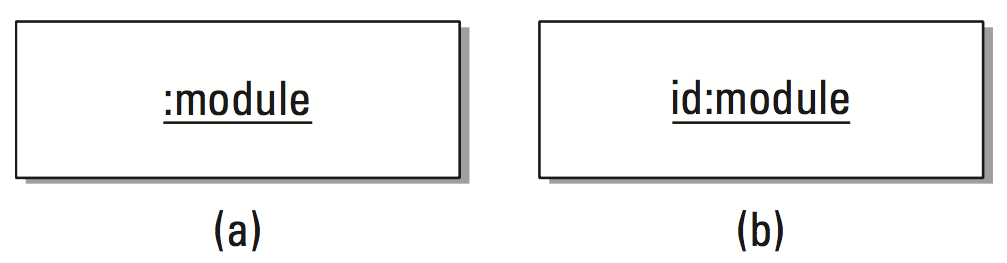
\includegraphics[width=0.5\textwidth]{img/f3-2.png}

	\caption{}

	\label{fig:f3-2}

\end{figure}



\begin{figure}[H] \centering

	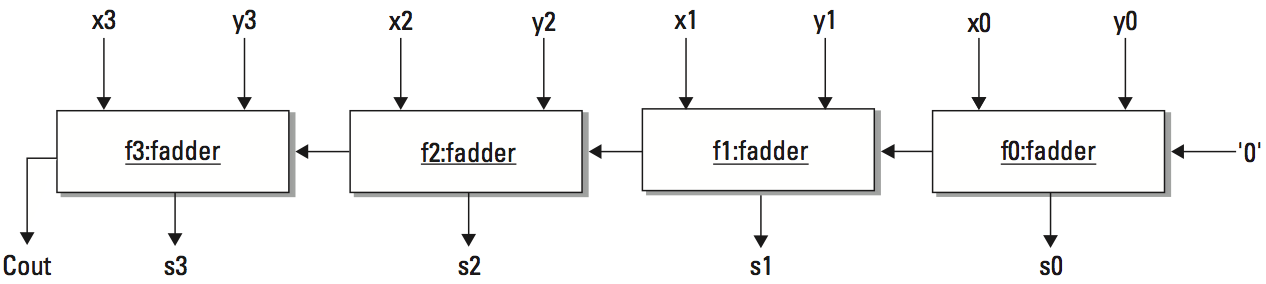
\includegraphics[width=0.5\textwidth]{img/f3-3.png}

	\caption{}

	\label{fig:f3-3}

\end{figure}



Tendo em mente todos estes conceitos, é possível descrever conceitos mais amplos no tema de \textit{design} de sistema.





\subsection{Abstração e Estado}



Abstração é definido no dicionário como operação intelectual em que um objeto de reflexão é isolado de fatores que comumente lhe estão relacionados na realidade, ou seja, tirar fora, extrair, remover. Assim, uma abstração é a arte ou um artifício de abstrair ou retirar. Dessa forma, um módulo é uma abstração de alguma funcionalidade em um sistema. Um módulo se torna uma boa abstração se suas interfaces e descrições provêm um fácil compreensão. Mas isso torna sua implementação mais complexa. Uma boa abstração capta todas características importantes e elimina tudo que não é importante para a ideia, ou seja cria uma organização. Uma imagem rica em informação pode não ser tão relevante imediatamente. Se isso for uma abstração ruim de algo, forçará-nos a pensar não sobre a singularidade do módulo, mas também como foi implementado, o que não é uma informação valiosa para uma abstração.

Estado já são uma palavra bastante conhecida no âmbito de sistemas eletrônicos. Eles são explicitados num \textit{design} de máquinas sequenciais e podem ser um ponto de memória de dispositivos eletrônicos como flip-flops. Já em sistemas embarcados, sua definição é um pouco mais abstrata já que um estado de módulo pode ser armazenado em vários lugares em várias formas distintas como flip-flops, static RAM, arquivo, ou até mesmo off-chip. Sendo assim, estado é uma condição de memória onde é possível segurar uma informação por um certo período de tempo.





\subsection{Coesão e Acoplamento}



Dessa forma, pra conceitos temos abstração e estado e pra mensuração teremos coesão e acoplamento. Coesão é uma métrica de abstração. Se os detalhes dentro de um módulo no ato da implementação são funcionalidades compreendidas facilmente, então o módulo possui coesão. O acoplamento é a forma de como os módulos estão relacionados uns com os outros. Uma dependência entre módulos é quando um comunica diretamente com outro. Quando um módulo A invoca um módulo B, então A depende de B. Mas B não necessariamente depende de A. Entretanto, dependência não é sempre explícita e com isso a o conceito estado entra em ação para auxiliar na formação de um módulo. Um exemplo disso é quando dois módulos parecem não ter nenhuma dependência entre si, mas que o sistema exige que ambos tenham terminado uma tarefa no mesmo tempo, criando assim uma dependência e consequentemente o sistema é acoplado no quesito tempo. Dependências não é algo ruim. São necessárias para que o procedimento possa funcionar corretamente com todos os outros módulos, mas precisa-se saber também o grau de acoplamento no sistema sendo essa em número e tipo. Dependência surgidas a partir de interfaces formais são as melhores formas de dependências. Uma forma de reduzir acoplamento em sistemas são por meio de encapsulamentos. Tais envolvem manipulações de estado e introdução à interface formal. A ideia é mover um estado dentro de um módulo e fazer com que isso seja exclusivo dele, também chamado de informação escondida. Isso permite uma maior liberdade de mudança interna no módulo já que a mudança de formatos de um estado não introduz um erro em outro e se o módulo possui uma boa abstração, então a informação escondida também permite que ele seja implementado de forma isolada. Assim, acoplamento é o resultado de dependências entre módulos.

É preciso evitar acoplamentos quando desnecessário e para isso existem várias técnicas para manipulação do grau de acoplamento.

É possível ver na Figura \ref{fig:f3-4} (a) que os submódulos B e C possuem dependência do módulo somatório A. Na Figura \ref{fig:f3-4} (b) a somatória A é duplicada dentro de cada submódulo eliminando cada uma das dependências existentes.



\begin{figure}[H] \centering

	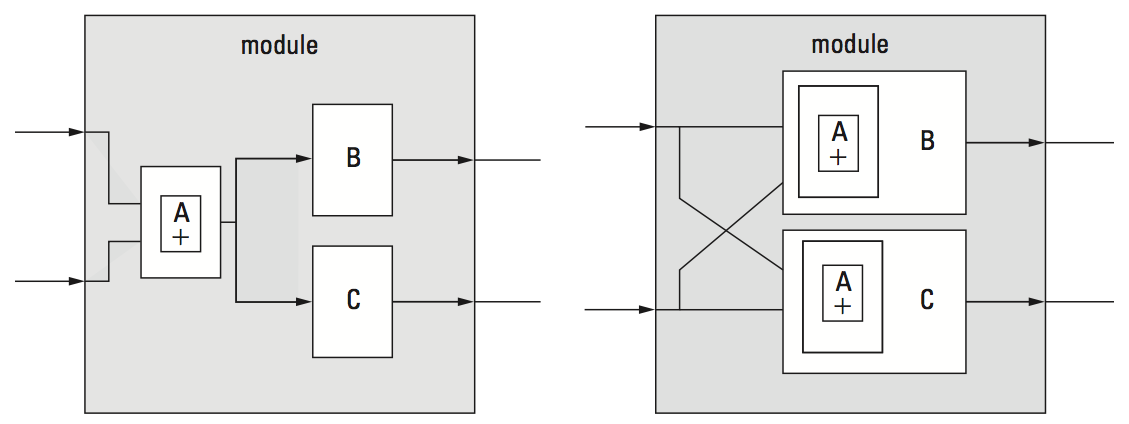
\includegraphics[width=0.5\textwidth]{img/f3-4.png}

	\caption{}

	\label{fig:f3-4}

\end{figure}



Será proposta uma situação exibindo o porquê desta abordagem pode ter mais vantagens: suponha que A foi \textit{design}ado para calcular somente números não-sinalizados. Mas com o passar do tempo, C necessita de operar com número sinalizados. Dessa forma, na Figura xa o \textit{design} deveria alterar tanto C quanto A. Alterando A, obrigatoriamente afetará B. Mesmo que B continue a trabalhar bem com a alteração de A, ouve uma cascata de alterações a serem feitas ao longo do tempo sobre algo que deveria ser pequeno, simples e isolado.

Discutindo sobre desvantagens deste procedimento, talvez se pensa que isso pode aumentar no tamanho do \textit{design} do projeto já que está duplicando um item, mas não. É possível que a funcionalidade de A seja simplesmente mesclado com o configurable logic block (CLB) já alocado para os submódulos B e C e consequentemente é possível que não haja nenhum ganho de conexão no CLB alocado. É claro que isso não é sempre verdade e é possível sim que tenha aumento de custo. Uma segunda desvantagem é, ao duplicar um módulo, agora se tem o mesmo componente em dois lugares. Se um erro for encontrado em um, deverá ser alterado noutro também.





\subsection{Planejando para o Reuso}



Além de qualidade, outro princípio é o torná-lo reusável. Com o constante aumento de complexidade dos componentes, é imprescindível que construamos \textit{design}s com intenção de serem reutilizáveis. Primeiramente é necessário criar e identificar \textit{design}s reutilizáveis. Alta coesão e baixo acoplamento são indicativos de componentes reutilizáveis. Existem custos em escondidos por meio de relative cost of reuse (RCR) e relative cost of writing for reuse (RCWR) e eles serão dissertados a seguir.

RCR são custos que fazem com que tenhamos que ler a documentação para entender como utilizar o módulo e o RCWR é o esforço extra que alguém deve exercer para projetar um módulo que outros possam utilizar (POULIN ET AL, 1993). Um exemplo é o \textit{trade-off} de aprender a utilizar a função strcpy da biblioteca string.h contra o tempo de criar a nossa própria função de cópia. Em alguns casos, poderia ser fácil gerar nosso próprio a invés de aprender um componente potencialmente complexo. Isso provavelmente seria por causa do alto RCR do módulo.

Uma forma de gerenciar o RCWR é tomar uma abordagem incremental onde é projetado um componente específico no \textit{design} atual. Se ele for necessário novamente, copie e generalize-o. Para vários \textit{design}s, adicionar uma generalização torna o componente reusável. Em linguagem VHDL, isso pode ser conseguindo introduzindo generics no projeto. Um ponto importante de máquinas computacionais personalizadas são a vantagem de serem específicas. Simplesmente adicionando generalização sem deixar a opção de gerar versões específicas de aplicativos através de genéricos é improdutivo. Refatoração é a tarefa de procurar em um \textit{design} existente e rearranjar os agrupamentos e hierarquia sem alterar sua funcionalidade, como é exibido muito bem na Figura \ref{fig:f3-4} e é feito para fazer componentes reutilizáveis. É possível que haja situações onde a refatoração pode acidentalmente alterar a sua funcionalidade. Para isso existe o processo de teste regressivo. Ele é usado para prevenir tal situação. Geralmente é automatizado e ser uma simulação dirigida tal como os testsbenchs já comumente conhecidos ou mesmo uma série de sistemas que contornam o componente exercitando sua própria funcionalidade. São necessários vários sistemas pelo fato de quererem também testar todos os genéricos que estão no conjunto em tempo de compilação.





\section{Gráfico de Controle de Fluxo}



É possível ver que os detalhes abordados aqui são referenciados a um \textit{design} de \textit{software}. É possível representar um sistema, quanto em \textit{software} ou em \textit{hardware}, de várias formas. Uma delas é o desenvolvimento de rápidos protótipos e este é referenciado como um \textit{design} de referencia de \textit{software}. Por mais que o custo de sua criação é algo ruim, sua forma de especificação sistêmica traz várias vantagens. A mais notável é a generalização de uma especificação bastante completa, sendo qualquer dúvida sobre o comportamento do sistema, é possível olhar no \textit{design} referencial. E sendo é um projeto que pode ser lido pelo computador, a sua especificação pode ser analisada por ferramentas computacionais.

Assumindo que o \textit{design} de referência de \textit{software} já exista, será mostrado como este pode ser demonstrado matematicamente e auxiliar-nos em o que deve ser implementado em nível de \textit{hardware} ou \textit{software}. Pra isso, utilizar-se-á o gráfico de controle de fluxo (CFG). Ele é definido por $ G = (V, E) $ onde V são vértices que representam os blocos básicos e as arestas indicam a todas as possibilidades de caminhos. Um bloco básico é uma sequência maximal de instruções sequenciais com \textit{single entry and single exit} (SESE).



\begin{figure}[H] \centering

	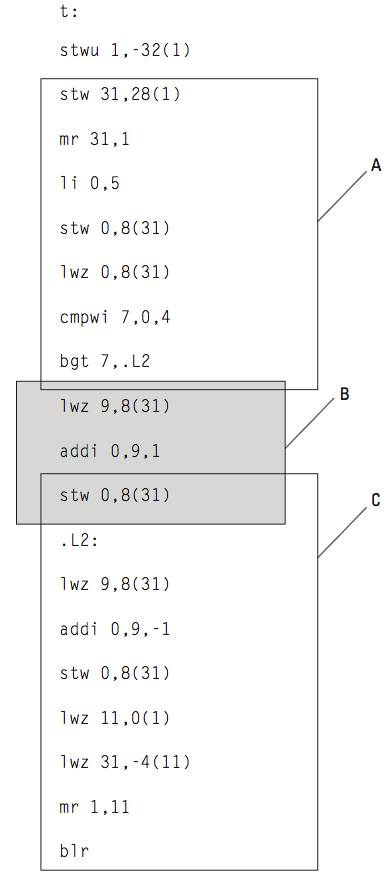
\includegraphics[width=0.5\textwidth]{img/f3-5.png}

	\caption{}

	\label{fig:f3-5}

\end{figure}



O primeiro grupo A é um bloco não básico porque não é maximal, ou seja, a primeira instrução store word with update deveria estar incluída. Grupo B é um bloco básico. Já o grupo C não é pois tem duas entradas para o bloco sendo elas no store word e também pelo branching para L2.



\begin{figure}[H] \centering

	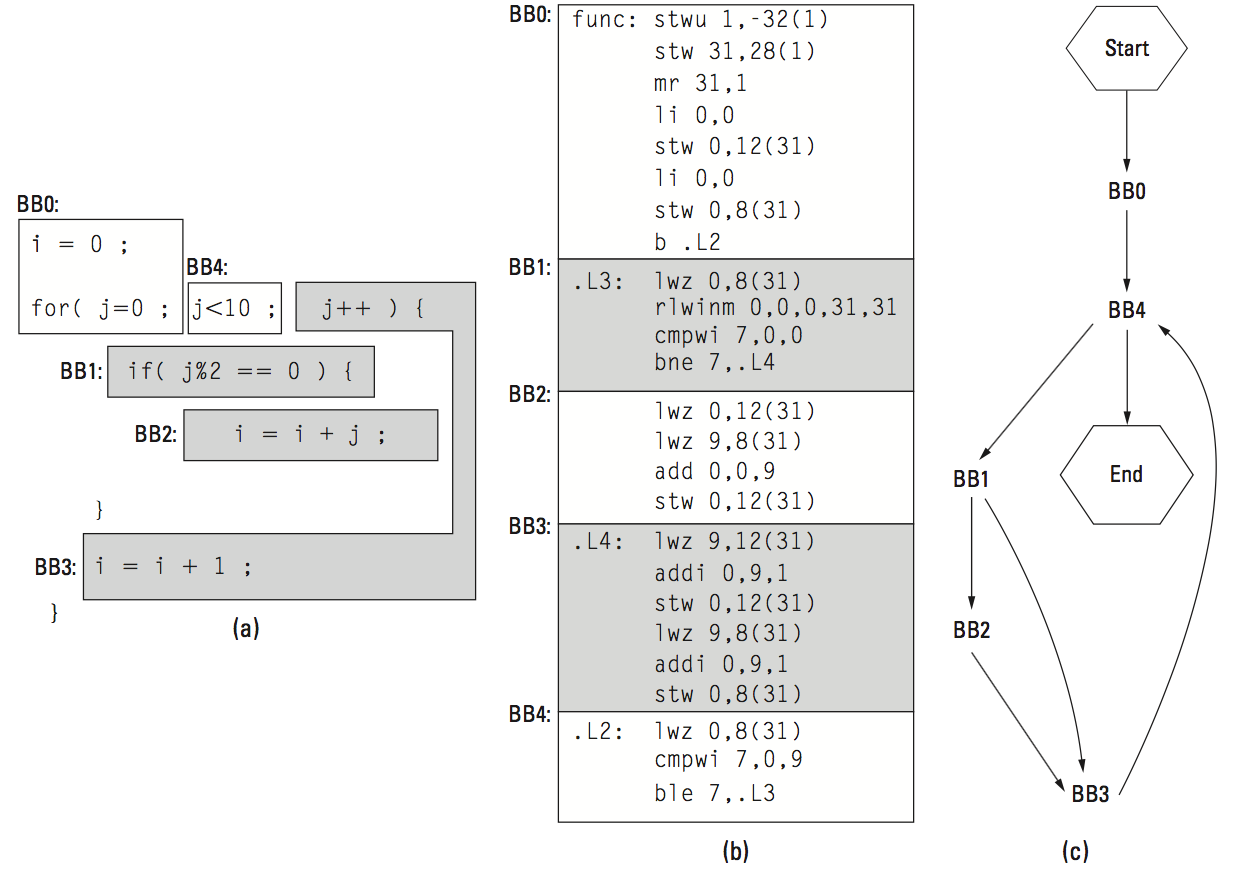
\includegraphics[width=0.5\textwidth]{img/f3-6.png}

	\caption{}

	\label{fig:f3-6}

\end{figure}



A Figura \ref{fig:f3-6} (a) exibe os blocos básicos em um código em alto nível. A Figura \ref{fig:f3-6} (b) exibe os o código gerado por um compilador para PowerPC onde os blocos básicos também são identificados e por fim o gráfico de controle de fluxo. Sabe-se que, é só possível identificar o bloco básico em C desde que se sabe como compilador foi  utilizado para gerar código, o que não acontece com assembly já que é possível identificar os blocos já com as próprias instruções.





\section{Design de \textit{Hardware}}



Até agora foi discutido os tópicos de modo genérico. A partir de agora, a discussão terá foco em \textit{design} em \textit{hardware}, em especial \textit{design} à Plataforma FPGA.

Designers raramente queriam construir em sistemas embarcados a partir de simples rabiscos e para isso utilizavam arquiteturas já existentes removendo componentes desnecessários e então adicionando cores aos requisitos do projetos. O modelo processador-memória, exibido na Figura \ref{fig:f3-8}, teve grande sucesso no início. Isso se tornou possível por causa da popularização do IBM Personal Computer em 80. Isso impulsionou desenvolvedores terceiros a criarem periféricos e máquinas compatíveis com outros fabricantes. E como a demanda aumentava com o passar do tempo, foi possível que os fabricantes pudessem tentar diferentes \textit{design}s de arquiteturas de computadores.



\begin{figure}[H] \centering

	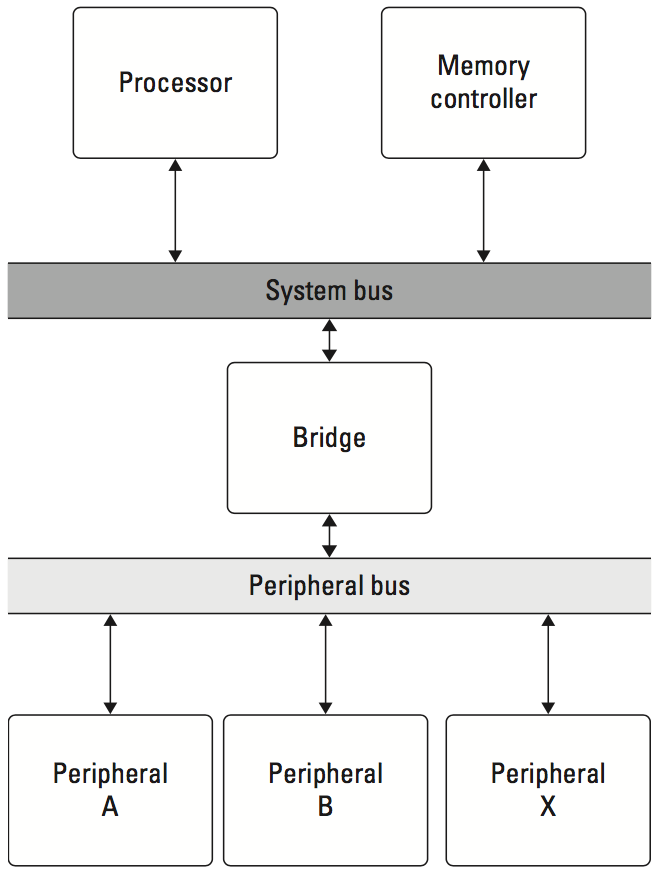
\includegraphics[width=0.5\textwidth]{img/f3-8.png}

	\caption{}

	\label{fig:f3-8}

\end{figure}



Computação embarcada não tinha grandes mudanças desde então, pois como é possível ver na Figura \ref{fig:f3-8}, esta arquitetura permitia o aprimoramento de componentes individuais do sistema. Por mais que o sistema de barramento seja insuficiente, ele serve bem para aplicações em geral e esse sistema é um bom ponto inicial para um \textit{design} em Plataforma FPGA. A Plataforma FPGA tem adota este tipo de arquitetura pois provê um framework estável que pode ser construído sobre \textit{design}s customizados. É possível construir complexos sistemas utilizando componentes existentes e cores, e com tempo reduzido em relação a sistemas embarcados tradicionais.





\subsection{Componentes de uma Plataforma FPGA}



Com a ideia de modularidade, coesão, casamento de componentes e \textit{design}, queremos iniciar uma construção de um sistema base que pode ser reutilizado como ponto de partida para um projeto de sistema embarcado, sendo este o modelo processador-memória.

O processador oferece controle e um ambiente de \textit{design} familiar ao \textit{\textit{design}er}. Mesmo que use pouca ou nenhuma relação com processadores, é usado para uma rápida prototipação. Pode existir dois tipos de processadores, os processadores \textit{hardware} e \textit{software} core, sendo o processador hard já é bem conhecido. Algumas Plataformas FPGA provê recursos reconfiguráveis suficientes para que um processador \textit{soft} possa ser implementado em blocos lógicos. Eles fornecem flexibilidade e são naturalmente configuráveis. Inicialmente, mesmo processadores básicos, precisam de alguns recursos básicos e tal forma se chama stand-alone.

Antes da implementação de fato, é preciso verificar se o FPGA já possui um processador \textit{hardware}, se possui recursos suficientes para a implementação de um, qual o papel do processador e o \textit{software} será utilizado nele e isso será discutido ao decorrer deste.

A memória pode ser organizada e hierarquizada de várias formas diferentes como Von Neumann ou Harvard, ou mesmo com níveis de caches diferentes. Tal como o processador, deve-se perguntar que tipos de memórias estão disponíveis, quanto há disponível e outros parâmetros de implementação. Em um sistema, ela pode ser considerada como um componente, um core, ou uma parte básica e sua localização determina a interface e acessibilidade. Um controlador de memória é requerido para controlar as transações de memórias. O uso eficiente é o item mais crítico pois ela pode gerar lags com o processador.





\subsubsection{Barramento}



As interfaces de cada componente, como o processador e memória, se conectam via barramento padronizado. Um core que pode requisitar acesso é considerado barramento master, o que demonstra que nem todos os cores necessitam de ser master, o que tornam barramento \textit{slave}. Um barramento no FPGA é implementado em lógica configurável, o que torna um \textit{soft} core. Detalhes importantes são quais cores necessitam de comunicar diretamente, alguns comunicam mais frequentemente ou necessitam de uma alta vazão.

Geralmente, o barramento com maior vazão é o que fornece a conexão entre processador e controlador de memória e geralmente é o primeiro barramento a ser adicionado ao projeto. Um segundo pode ser adicionado para separar o \textit{design} em diferentes domínios, geralmente em \textit{low} e \textit{high-speed} ou com largura de banda dedicada à comunicação. Esses são conhecidos como barramento de periféricos. Utilizando barramentos simples, para realizar uma operação na memória, deve-se realizar uma requisição e o múltiplos barramentos permitem a comunicação paralela.

Quando necessita de uma comunicação de um core com um periférico, utiliza-se de um bridge. É um core especial que resite em ambos os barramentos e propaga requisições de um barramento para outro. Trata-se de uma interface que funciona como um barramento mestre em um barramento e um barramento \textit{\textit{slave}} em outro e assim o \textit{\textit{slave}} responde à requisição que deve ser passada a outros os periféricos. Geralmente somente uma bridge simples é requerida, onde todos os periféricos são conectados nela, tendo um sistema de bridge para gerenciamento das solicitações e respostas.





\subsubsection{Periféricos}



Quando se menciona periféricos, geralmente é referido à \textit{hardware}s cores como impressoras, LCDs, GPSs e outros. Periféricos pode-se de dizer que são todos os componentes que estão em torno à unidade de processamento central. Todos eles possuem algum tipo de interface de comunicação, sendo ela uma PCI Bridge, Ethernet, USB, UART, I$^2$C, SPI e muitos outros.







\subsubsection{O Sistema Base}



Pra início, será montado um sistema conceitual simples constituído de um processador, dois tipos de memória e uma comunicação UART. Como resultado, este conceito será base para vários outros tipos de \textit{design}s.



\begin{figure}[H] \centering

	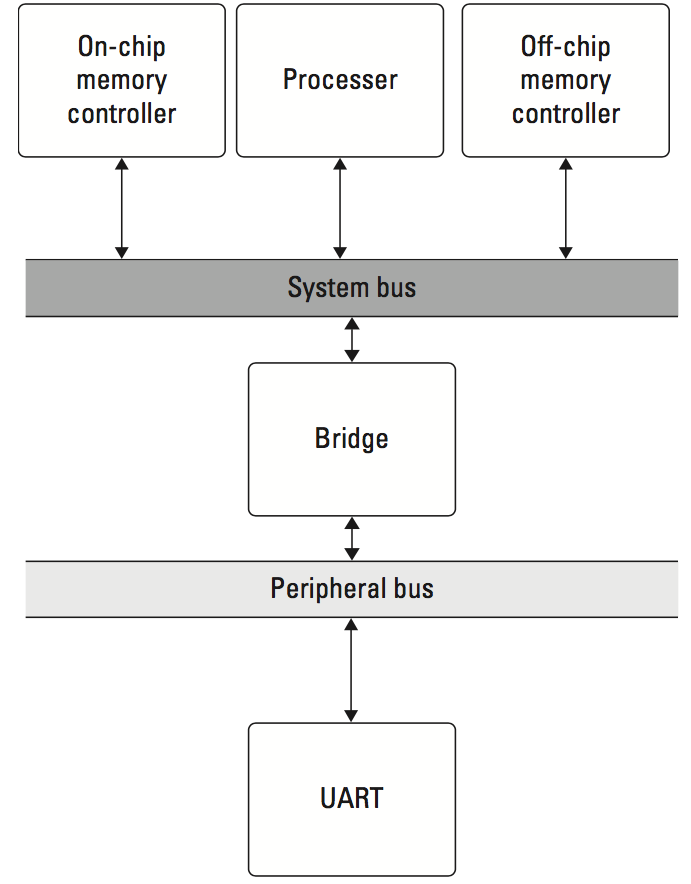
\includegraphics[width=0.5\textwidth]{img/f3-9.png}

	\caption{}

	\label{fig:f3-9}

\end{figure}



O benefício de utilizar dois sistemas de barramento é a facilidade de modificação ao adicionar e substituir componentes podendo assim termos o seguinte \textit{design} de sistema exibido na Figura \ref{fig:f3-10}, de acordo com nosso propósito.



\begin{figure}[H] \centering

	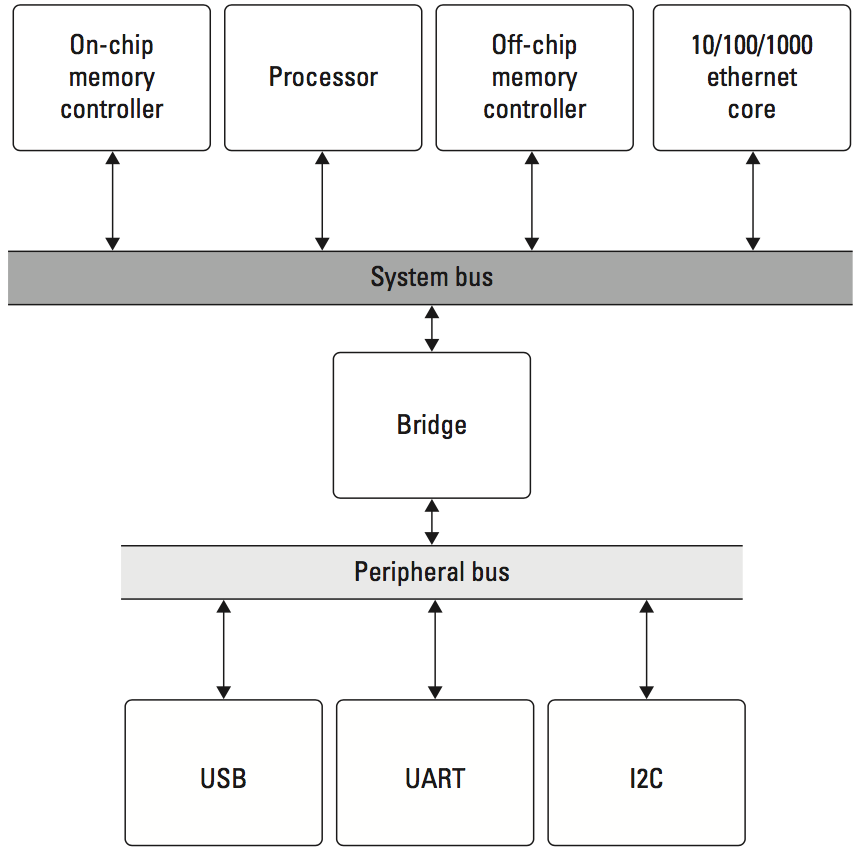
\includegraphics[width=0.5\textwidth]{img/f3-10.png}

	\caption{}

	\label{fig:f3-10}

\end{figure}



Em uma perspectiva de \textit{hardware}, a localização de dados é facilmente identificável. Memória off-chip é um modo separado e seu acesso é nada mais que seus endereços. O endereçamento é importante para qualquer core possa comunicar com o processador. A Figura \ref{fig:f3-11} mostra o mapa de endereçamento dos dois barramentos. Cara core possui um intervalo na memória é considerado um \textit{\textit{slave}} e o processador não possui um espaço de memória no mapa. Em sistemas com dois barramentos, o bridge atua como um intermediário entre as requisições e o sistema de barramento periférico.



\begin{figure}[H] \centering

	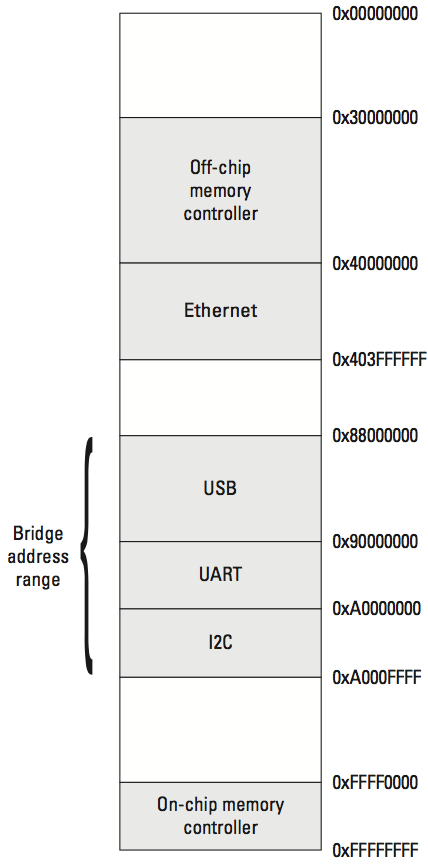
\includegraphics[width=0.5\textwidth]{img/f3-11.png}

	\caption{}

	\label{fig:f3-11}

\end{figure}



\subsection{Montando Sistemas Personalizados}



Para iniciar, deve-se responder a pergunta de porque construir um sistema personalizado. Acreditava-se que desenvolvimento de \textit{hardware} é um processo difícil porque existem mão de obra para \textit{software}s profissionais do que engenheiros de \textit{hardware}. E a resposta para a pergunta ‘porque desenvolver um \textit{hardware}’ é para obter performance além de eficiência e previsibilidade.

Sabendo-se que um FPGA não terá o mesmo ganho que um processador projetado já em silício, deve-se analisar como o \textit{hardware} FPGA supera um processador. Existem duas razões porque alguns \textit{design}s de FPGA possuem vantagens em performance. A primeira é sobre o modelo de execução. O modelo de computação sequencial von Neumann possui uma barreira em sua performance por causa do fato de expressar suas tarefas como um conjunto sequencial de operandos. Em \textit{hardware}, o paralelismo inerente da tarefa pode ser expressado diretamente. Para compensar sua operação serial inerente, processadores modernos possuem uma porção significante de recursos de \textit{hardware} para extrair em nível de instruções o paralelismo como estratégia de aumentar a vazão. Para algumas aplicações, largura de banda de memória limita a performance e parte da banda é consumida pelas instruções sendo buscadas, da memória e assim, instruções fazem parte implícita do \textit{design}. A segunda razão é que FPGA pode ter uma especialização. Em processadores de propósito \textit{data path} e tamanho de operações são organizados por meio de requerimentos gerais. Isso significa que, para multiplicar um inteiro por uma constante $ c $ é necessário de um multiplicador completo no sistema. Se essa informação já é conhecida, uma implementação baseada em FPGA pode ser criada com funções personalizadas.

Supondo que uma implementação em \textit{hardware} de uma tarefa A leva o mesmo tempo a ser executada no processador e ambas são de fácil implementação e questiona-se se ainda é viável a implementação desta. A resposta é sim quando a solução em \textit{hardware} é mais eficiente. Eficiência é definida como facilidade de realizar uma tarefa fixa com uma quantidade variável de recurso sendo recurso a área de prototipação, número discreto de chips, ou o custo da solução. Um \textit{hardware} personalizado e um processador possuem são mais eficientes que dois processadores.

É possível também o caso de um processador não ser totalmente utilizado de sua capacidade. Mesmo utilizando a propriedade de multitarefa em novas funcionalidades, existem razões para escolher a implementação. Alguns casos faz sentido mover uma tarefa para o \textit{hardware} se a torna mais previsível ou se torna o escalonamento no processador mais facilitado. Em casos onde restrição de tempo é importante, como sistemas de tempo real, a meta é satisfazer as restrições e assim previsibilidade é mais importante que performance. Entretanto, a única desvantagem de desenvolver em \textit{hardware}, como já mencionado é o esforço requerido. O número de engenheiros de \textit{hardware} é relativamente baixo comparado com profissionais que desenvolvem em \textit{software}. Desenvolvimento em \textit{hardware} não mais difícil que em \textit{software}, mas sim, necessita de atenção no projeto. Em resumo, uma Plataforma FPGA oferece vantagens de performance, eficiência e previsibilidade sobre soluções somente em \textit{software}. Como um projetista de FPGA, parte de sua tarefa inclui determinar quando um simples controlador é apropriado.



\subsubsection{Composição de \textit{design}}



Existem três passos para fazer um \textit{design} de um core modular customizado. O primeiro passo é identificar as entradas e saídas, onde em muitos casos estas são baseadas em suas funcionalidades. O segundo é identificar os operandos e compor o \textit{data path}, geralmente uma coleção de computações de multiestágios (isto é, \textit{pipeline}). Cada componente é \textit{design}ado a uma funcionalidade particular. Os operando exatos podem não ser claros no início da fase de \textit{design}, mas determinando a funcionalidade em baixo nível necessárias permite a construção de um \textit{data path}. Um \textit{data path} representa o fluxo de dados por meio do componente. Uma vez definido, é possível construir o \textit{pipeline}, no qual contribui com a performance e eficiência do \textit{design}. Capturando os estágios do \textit{pipeline} pode ser árduo inicialmente, mas iniciando um \textit{design} com o conceito de suporta à operações \textit{pipeline} faz com que o projeto seja mais gerenciável. O terceiro paço é o desenvolver o circuito de controle que sequencia as operações, frequentemente a máquina de estados finitos. Frequentemente referenciamos um \textit{hardware} em termos de paralelismo, onde cada operação é independente e podem ser executadas ao mesmo tempo. Com a máquina de estados finitos é possível gerenciar a computação executando as operações paralelas e em seguida as sequencias e dependentes.

Existem duas abordagens de \textit{design}, \textit{bottom-up} e \textit{top-down}. Em muitos casos, utiliza-se a abordagem \textit{bottom-up} no desenvolvimento em FPGA. Em método estrutural HDL, cada componente é construído por seus subcomponentes e assim, antes do \textit{top-level}, todos os subcomponentes devem ser construídos e testados. Nessa abordagem, cada subcomponente pode ser tratado como uma \textit{black-box} onde as entradas e saídas são conhecidas. Na abordagem \textit{top-down}, quando se quer desenvolver um core personalizado, o \textit{\textit{design}er} deve começar com as interfaces de entrada e saída, criando assim o início da \textit{black-box}. Uma vez definida, é possível decompor sistematicamente em subcomponentes. Esse processo repete até os blocos de baixo nível onde podem ser simples o suficiente. Esta abordagem não é associada a nenhum HDL estrutural ou comportamental, mas é possível utilizada com o último.

Em ambas as abordagens, internamente podem ser construídas de formas distintas, mas no final todas possuem a mesma funcionalidade. Considere o seguinte componente somador de quatro números da Figura \ref{fig:f3-12}. Na implementação temporal da Figura \ref{fig:f3-13} existe um multiplexador que realizará a soma de acordo com o controlador da máquina de estados finitos. A máquina de estados finitos terá quatro estados ao todo e percorrerá de forma sequencial. Utilizando somente uma ALU e um registrador, temos o circuito que utiliza menor quantidade de recursos possível, mas não temos a solução com menor tempo. Para aumentar o speed-up, devemos considerar a abordagem paralela e adicionar mais recursos. Um sistema com três ALUs poderá realizar as operações \texttt{temp1 = a + b}, \texttt{temp2 = c + d} e \texttt{temp1 + temp2}. O \textit{trade-off}, da latência e recursos fica a cargo do \textit{\textit{design}er}.



\begin{figure}[H] \centering

	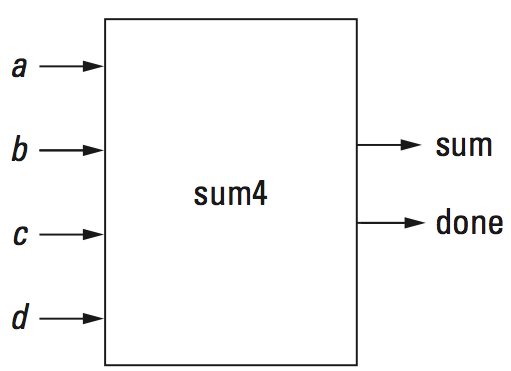
\includegraphics[width=0.5\textwidth]{img/f3-12.png}

	\caption{}

	\label{fig:f3-12}

\end{figure}



\begin{figure}[H] \centering

	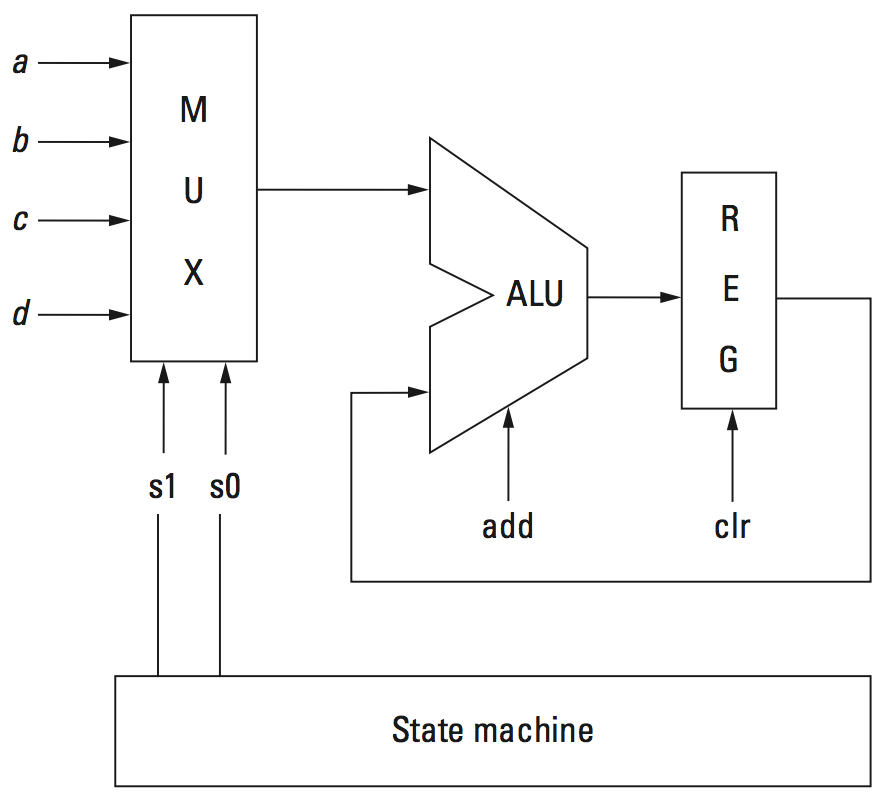
\includegraphics[width=0.5\textwidth]{img/f3-13.png}

	\caption{}

	\label{fig:f3-13}

\end{figure}



Quando existem operações sequencias, implica que existe um controle onde a segunda toma lugar em seguida da primeira após sua computação e isso degrada no caso de composição espacial o que diminui a estrita ordenação de operações. Dessa forma, quando um \textit{hardware} especifica duas operações, elas serão executadas simultaneamente ao menos que o \textit{\textit{design}er} tenha especificado previamente uma ordem. A Figura \ref{fig:f3-14} mostra a implementação espacial do somador. Nesse caso, as operações de adição são \textit{pipeline} tais que os resultados são alimentados para frente para o próximo somador. E execução solta em FPGA pode gerar vantagens e desvantagens. A concorrência é o que fornece ao sistema performance, e controle do tempo é o que fornece previsibilidade. Expressar simplesmente relações de tempo entre operações é um desafio.



\begin{figure}[H] \centering

	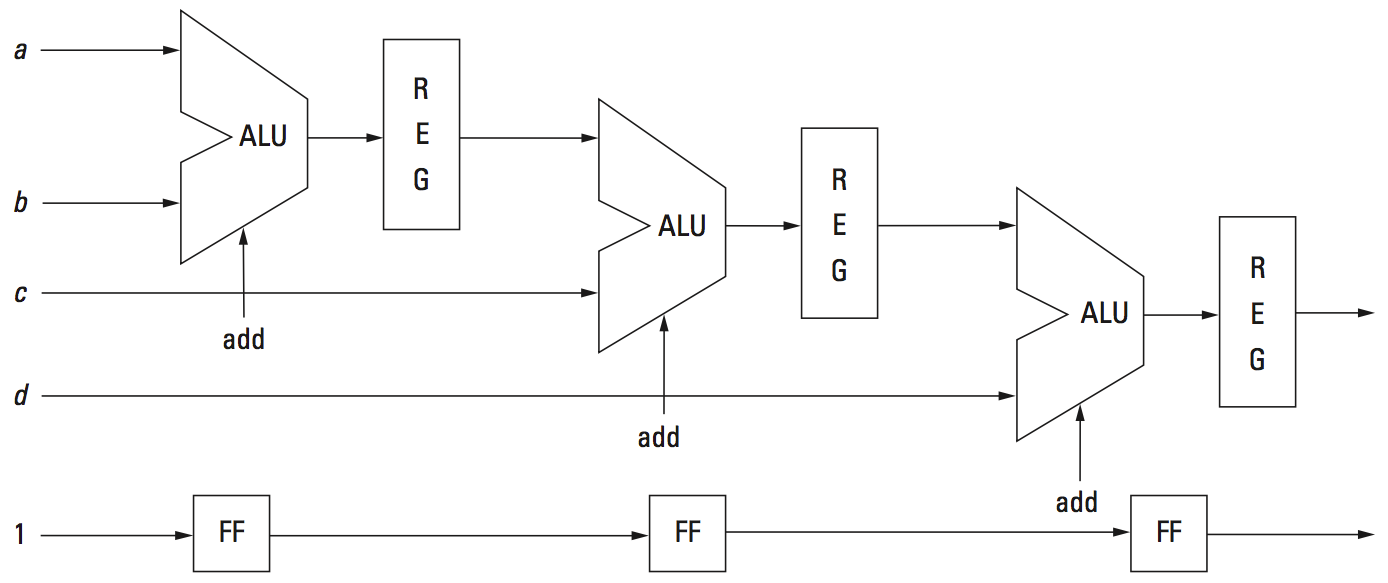
\includegraphics[width=0.5\textwidth]{img/f3-14.png}

	\caption{}

	\label{fig:f3-14}

\end{figure}



\section{Design de Software}



No passado, \textit{software} era simples. Tinham uma simples tarefa, e executava um papel relativamente menor comparado com o \textit{design} de \textit{software} da época. Se duas tarefas eram solicitadas, eram frequentemente deixadas independentes, lógico e fisicamente. Com microcontroladores tornando mais veloz, sistemas embarcados adicionaram sistemas de \textit{software} para gerenciar controle de múltiplas tarefas. Isso permite quem um microcontrolador simples possa fazer a multiplexação de tarefas separadas por tempo. Em sistemas embutidos atuais, seus processadores possuem unidade de gerenciamento de memória, suporte de memória virtual e com tecnologia suficiente para suportar sistemas operacionais. Tais características são tidas como vantagens pois resulta em uma explosão de novas características e assim permitindo a incorporação e adaptação de aplicações de \textit{software}s grandes que originalmente eram escritos para computadores de propósito geral e máquinas servidoras.





\subsection{Opções de Sistema de Software}



Um desenvolvimento de um sistema embarcado possui vasto escolhas quando vem para sistema de \textit{software}. Sistema de Software referimos a qualquer \textit{software} que assista a aplicação, geralmente adicionando uma interface em \textit{software} para acesso ao \textit{hardware}. Isso segue desde simples bibliotecas de rotinas até sistemas operacionais totalmente desenvolvidos que virtualizam o \textit{hardware} para processos individuais. Em muitos os casos, não é necessário um sistema de \textit{software}. Nesses casos, os arquivos iniciais executados antes do \texttt{main} em C, por exemplo, são modificados. Sem um sistema operacional, essas rotinas são responsáveis por definir o estado inicial do processador e periféricos. Mesmo que o processador tenha uma unidade de controle de memória,  simples casos que a aplicação executa em modo real e privilegiado, nenhuma proteção de memória é utilizado. Isso se chama programa standalone C, pois executa sem nenhum sistema de \textit{software} adicional e com isso, tem uma abordagem de sistema simples.

Para FPGA, isso é frequentemente o primeiro passo quando se testa um novo \textit{hardware} core, pois um programa em C tem total acesso ao \textit{hardware}. Geralmente, essa solução produz um executável suficientemente pequeno que o sistema de \textit{software} inteiro pode ajustar dentro de um bloco de memória RAM no FPGA. A desvantagem é a necessidade de desenvolvimento. Não á proteção contra erros de \textit{software}. Talvez o grande retrocesso hoje é que é difícil ter vantagem de \textit{software} existente que assume que admite uma biblioteca C completa e um \textit{workstation}. As vezes a adição de funcionalidades de um sistema de \textit{software} como o suporte a multithreads pode ser útil, diferente da indesejável sobrecarga ao adicionar recursos completos de um sistema operacional. Vários produtos e soluções Open-Source são feitos para sistemas embutidos.

Um passo acima de standalone é uma simples biblioteca de threads. Sistemas operacionais provem um número de serviços para uma aplicação, mas isso tem um custo. Os sistemas operacionais de sistemas embarcados são diferentes dos utilizados nos desktops, significando que o desenvolvedor tem que aprender novas interfaces, convenções e o que está ou não disponível. Analisando de forma espectral, em um lado tem-se um sistema operacional com recursos completos, utilizados por \textit{\textit{workstation}s}. A maioria dos sistemas de \textit{software} descritos podem ser executados sem um subsistema de armazenamento secundário, ou seja, um sistema de arquivo. Entretanto, sistemas completos necessitam, no mínimo, sistema de arquivo raiz. Até recentemente, era inviável pensar em um sistema operacional completo em um sistema embarcado por causa de recursos requeridos. Entretanto, com novos dispositivos como a Plataforma FPGA isso se torna mais comum. Quanto mais serviços é colocado mais peso é adicionado ao desenvolvedor em saber o que é provido num sistema de \textit{software} e saber usá-lo. Com sistemas completos, os programadores já estão familiarizados com estes. Como sistemas operacionais são comuns, existem várias aplicações disponíveis. Com os sistemas embarcados se tornando mais obliquo e conectado à internet, eles necessitam suportar mais interfaces e mais protocolos de comunicação, o que o sistema operacional completo já fornece.



\subsection{Monitores e Bootloaders}



Nos primeiros microprocessadores baseado em sistemas embarcados, simples 8-bit migraram de computadores de hobbies e games para outros produtos comercias que agora chamamos de sistemas embarcados. Fabricantes desses microprocessadores geralmente desenvolvem kits que incluem board fabricadas que aumentam as capacidades dos chips e uma Board Support Package (BSP) que inclui compiladores, \textit{software} power-on-self-test (POST), bibliotecas de \textit{software} de Basic Input/Output System (BIOS) e um debugger. POST é executado antes de qualquer outro \textit{software} para verificações de que nada foi esgotado desde a última vez que foi ligado. Usando sub-rotinas da BIOS, o tamanho da aplicação continua pequeno.

Monitor é um simples \textit{software} de tipo primitivo ao debug. Debuggers modernos executam em um processo separado, tem acesso à tabela de símbolos do compilador e fornece uma rica e flexível interface. Ao contrário, um monitor é um driver de interrupção e suporta algumas funcionalidades básicas. Monitores tinham uma funcionalidade que não existem nos debuggers atuais, no qual suporta a transferência de memória sobre canal de comunicação serial transmitindo ASCII usado para interação. Como os caracteres ASCII possuem 7 bits e executáveis utilizam tudo como 8-bits de um byte, blocos de memória foram codificados para a transmissão. Enquanto é desenvolvido a aplicação, o \textit{\textit{design}er} poderia iniciar o monitor e copiar a aplicação para a RAM, ajudando o curto teste/debug dos \textit{software}s. Isso é importante pois, até o GNU debugger (ou gdb) possui subsistemas capazes de comportar como monitores.

Sistemas modernos moveram um passo a diante. Uma moderna substituição de um monitor pode ser a interface joint test action group (JTAG). Tal controlador gerencia qualquer endereço físico, incluindo a memória principal, provendo uma alternativa a abordagem dita dos monitores. Nesse caso, o debugger comunica com uma interface até o controlador JTAG. Da mesma forma as funcionalidades de POST/BIOS tem transformado em \textit{software} BIOS de desktops no qual inicia logo em seguida da energização do computador. Para alguns computadores, é critico que o BIOS coloque o computador e seus periféricos em um estado conhecido. Linux por exemplo não assume nada e permite que cada \textit{hardware} inicialize sozinho. Parcialmente concorrente com o desenvolvimento de PC, \textit{\textit{workstation}s} surgem com uma abordagem levemente diferente. Elas utilizam um pequeno \textit{software} chamado bootloader ou também chamado de PROM. Era simplesmente um programa que lia o primeiro setor de um disco, no qual contia outros programas mais avançados, e carregava-os para a memória principal, apontando o PC para o primeiro endereço desse setor. Esse então processava o carregamento do sistema operacional por completo. Essa técnica vem surgindo em PCs com boa aceitação. BIOS continua sendo o primeiro a ser executado, então o bootstrap é iniciado carregando o sistema operacional. Alguns conhecidos hoje são GRUB, U-Boot e o RedBoot.

Para sistemas embarcados, a abordagem BIOS/monitor ainda domina os pequenos microcontroladores e o legado sistêmico enquanto o bootloader está ganhando espaço em sistemas operacionais completos.



\part{Capítulo 4 - Problema de Particionamento}


%\section{Códigos}
	\subsection{Código em Linguagem Arduino}
	\begin{minted}
		[
		frame=lines,
		framesep=2mm,
		tabsize=3,
		breaklines=true,
		baselinestretch=1.2,
		fontsize=\scriptsize,
		linenos
		]{C}
		
		// Cálculos usados para calcular média
		long media_sensores;
		int somatorio_sensores;
		
		// Posicao do veículo
		int posicao;
		
		int quant_sensores = 6;
		long sensores[]    = {0, 0, 0, 0, 0, 0};
		
		void setup(){
			Serial.begin(9600);
		}
		
		void loop(){
			leitura_sensores();                      // Reads sensor values and computes sensor sum and weighted average
			calculo_proporcao();                     //Calculates posicao[set point] and computes Kp,Ki and Kd
			calculo_giro();                          //Computes the error to be corrected
			atuacao_motor(velocidade_direito, velocidade_esquerdo);  //Sends PWM signals to the motors
		}
	
		void leitura_sensores() {
			media_sensores     = 0;
			somatorio_sensores = 0;
			for (int i = 0; i < quant_sensores; i++){
				sensores[i] = analogRead(i);
				
				media_sensores += sensores[i] * i * 1000;     //Calculating the weighted mean of the sensor readings.
				somatorio_sensores += int(sensores[i]);       //Calculating sum of sensor readings.
				
			}
		}
	
		void calculo_proporcao(){
			posicao   = int(media_sensores / somatorio_sensores);
			proporcao = posicao – posicao_perfeita;      // Replace posicao_perfeita by your set point
			integral  = integral + proporcao;
			derivada  = proporcao - ultima_proporcao;
			ultima_proporcao = proporcao;
			
			valor_erro = int(proporcao * Kp + integral * Ki + derivada * Kd);
		}
	
		
		void calculo_giro(){  //Restricting the error value between +256.
			if (valor_erro< -256){ valor_erro = -256;     } if (valor_erro> 256){
				valor_erro = 256;
			}
			
			// If valor_erro is less than zero calculate right turn speed values
			if (valor_erro< 0){
				velocidade_direito  = velocidade_maxima + valor_erro;
				velocidade_esquerdo = velocidade_maxima;
			}
			
			// Ifvalor_erro is greater than zero calculate left turn values
			
			else{
				velocidade_direito  = velocidade_maxima;
				velocidade_esquerdo = velocidade_maxima - valor_erro;
			}
		}
	
	
		void atuacao_motor(intvelocidade_direito, intvelocidade_esquerdo){
			// Drive motors according to the calculated values for a turn
			analogWrite(motor_direito, velocidade_direito);
			analogWrite(motor_esquerdo, velocidade_esquerdo);
			delay(60);
		}
		
	\end{minted}

%@book{sass2010embedded,
%  title={Embedded systems design with platform FPGAs: principles and practices},
%  author={Sass, Ronald and Schmidt, Andrew G},
%  year={2010},
%  publisher={Morgan Kaufmann}
%}

\end{document}
